\chapter{Architecture}
\label{sec:architecture}
This chapter will give an overview of the general concepts that were followed in the implementation. Supplementary to this the core components of the application are introduced with some examples on how to use them.

\section{General concepts}
The complete code was structured with too general goals in mind. The first goal is that the application should be modular. This means it consists of components that can be reused on multiple occasions. For example a dialog for the deletion of an object can be always the same and only the internal handling and the displayed text have to be adapted based on the use case. This modularity will be introduced implicitly by React, because the general idea is the creation of components that will be updated internally by React.

Another relevant aspect was the future extension of the application, in order to be able to integrate more steps for the creation of the configuration. For example adding additional properties for the subcomponent configuration. React facilitates this, because it is possible to create extensible components that can be adapted in the future.

\section{App-Component}
The App is the central component that manages the application state and contains all the other components in the DOM after it is rendered. The App keeps track of the current configuration and provides access to it via a context provider\footnote{\url{https://reactjs.org/docs/context.html}}. This allows all components to access and update the configuration, which will also trigger the React lifecycle to re-render the current visible components.

\section{Welcome page}
The welcome page is the first component that is actually displayed when a user opens the application. Figure \ref{fig:app_welcome} show the welcome page that consists in general of two buttons. The "NEW CONFIGURATION"-Button starts the wizard (compare section \ref{sec:wizard}) to create a new configuration. The "LOAD CONFIGURATION"-Button starts the wizard, but will add an additional step that allows a user to import an existing configuration. This allows a user to update an existing configuration, for example with new subcomponents.

\begin{figure}[ht]
    \centering
    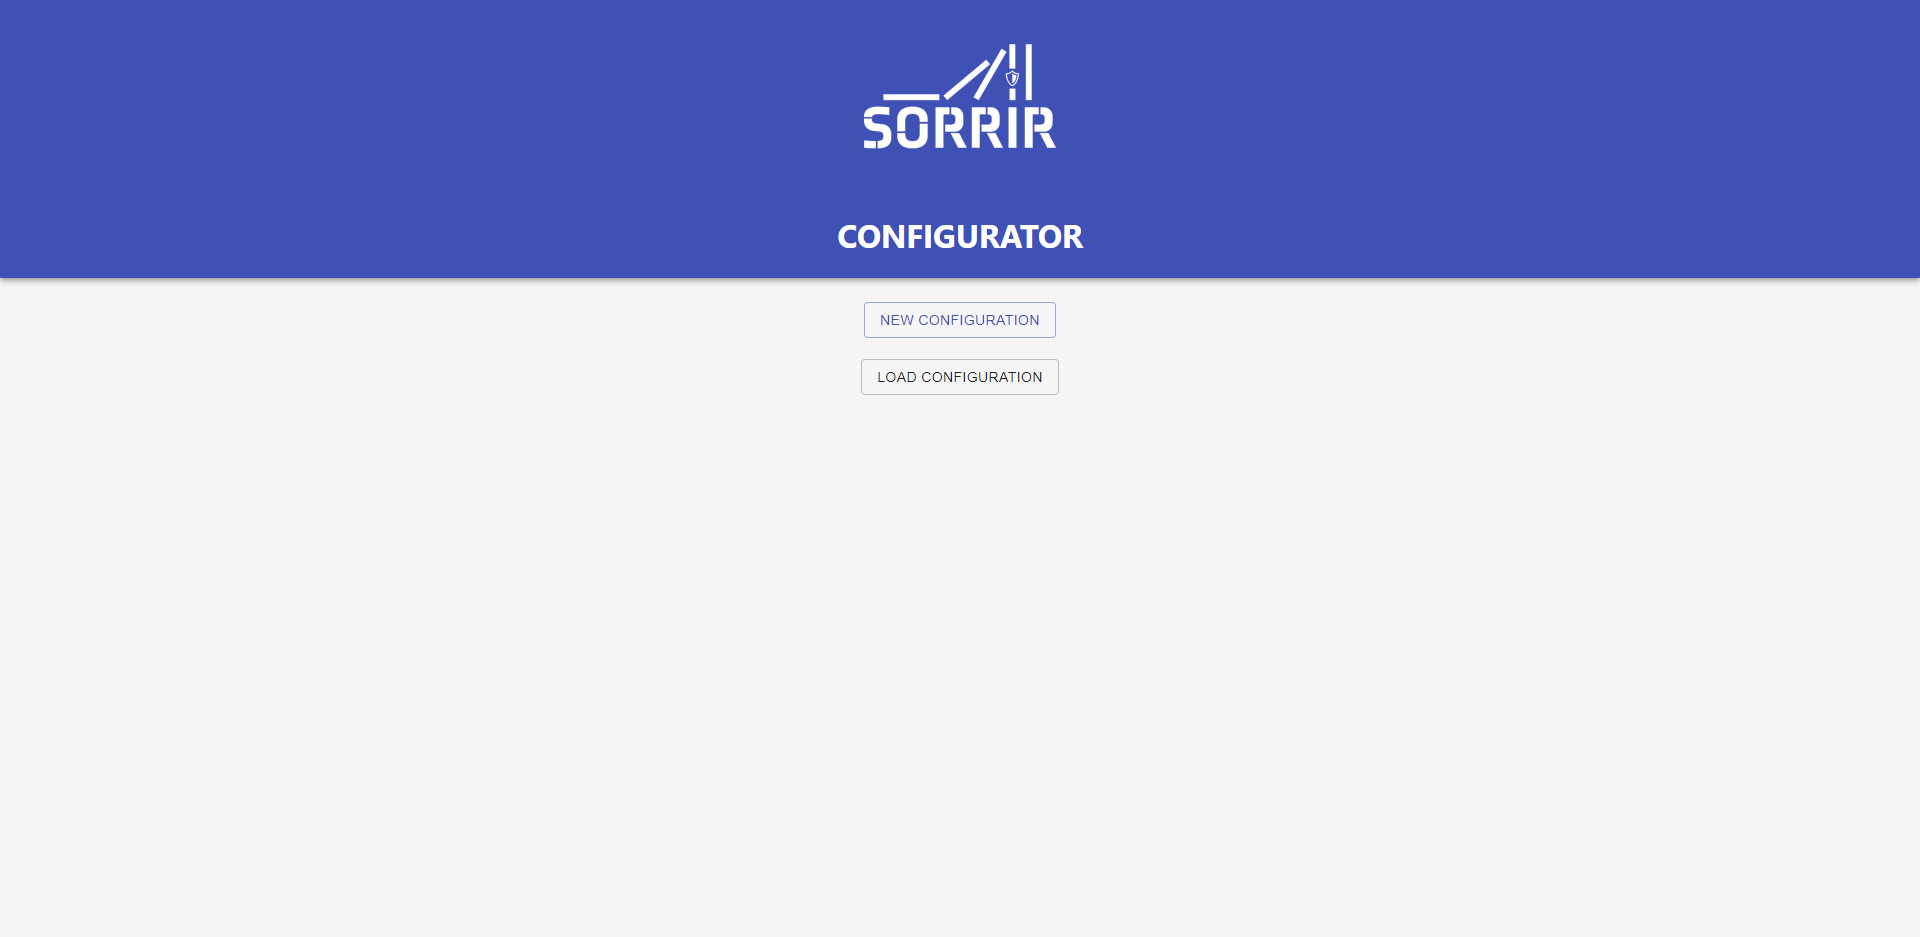
\includegraphics[width=\textwidth]{img/app_welcome.png}
    \caption{Welcome page}
    \label{fig:app_welcome}
\end{figure}

\section{Wizard}
\label{sec:wizard}
It is possible to divide the creation of a configuration into several steps. Displaying the steps separately to the user facilitates the configuration, because she is able to focus on one aspect at a time. To provide this functionality, a wizard was implemented that allows the step-by-step configuration. The wizard supports not only a linear configuration, which means each step after another step, but also to navigate arbitrary back and forth between the different steps of the configuration. 

The wizard component allows to dynamically configure the steps and their order. The wizard consist of a menu bar, a stepper and the content. The content can be any react component or HTML Tag and is internally called a view. 

Figure \ref{fig:wizard} shows the wizard for the configuration with an import. The menu bar is on the top of the website and updates its label with the label that was specified for the current step, for example in the figure the label was set to "Import". The menu bar contains a menu on the right that allows to display menu items that execute an action. The menu items represent global actions, that can be executed at any point in the configuration. At the moment the menu contains only one menu item that allows to restart the configuration, but it is possible to further add more functionality. The restart will show a dialog to confirm the reset of the current configuration and will, after the confirmation, send the user back to the welcome page.

The stepper is located underneath the menu bar and shows the individual steps of the configuration. The stepper highlights the current step and allows to navigate to any other step by clicking on it. The arbitrary navigation in the wizard also creates a constraint for the development of the different components that are displayed. It is necessary that each component that will update the global configuration has to leave the configuration in a valid state. For example a user creates a degradation level that depends on previous defined subcomponents. If she deletes one of these subcomponents afterwards the dependencies of the degradation level aren't valid anymore and therefore it is necessary to update the configuration or more precise the degradation level. 

\begin{figure}[ht]
    \centering
    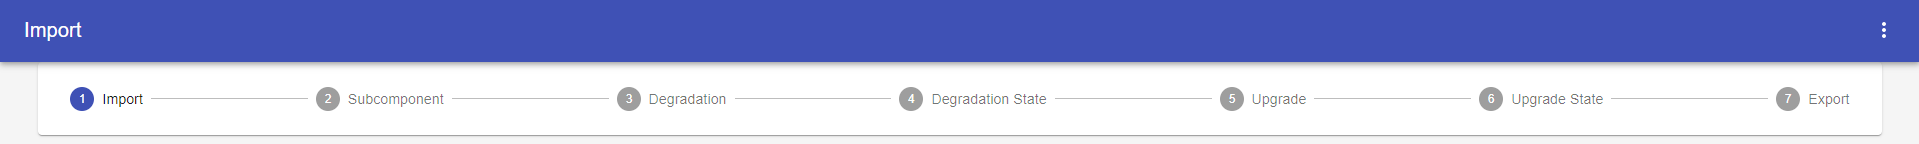
\includegraphics[width=\textwidth]{img/wizard.png}
    \caption{Wizard}
    \label{fig:wizard}
\end{figure}

\noindent In order to extend the wizard with additional or new steps following actions have to take place:

\begin{itemize}
    \item Extension of the view enum ( a enum that contains all available views in the application) ("src\textbackslash util\textbackslash Views.ts")
    \item Setting a label for the new view ("src\textbackslash util\textbackslash ViewLabelResolver.ts")
    \item Adding the view that will be displayed for the step in the wizard. This has to be a react component ("src\textbackslash components\textbackslash wizard\textbackslash ViewSelector\textbackslash ViewSelector.tsx")
\end{itemize}

\noindent After these steps the wizard can be configured to display the new view as an additional step. The view can then display any react component or valid HTML and has access to the configuration via the context from react. The only constraint for a fully functional view is to guarantee that any change of the configuration will leave the global configuration in a valid state.

\section{Import}
The import view is only inserted as a step when the wizard is started with the "LOAD CONFIGURATION"-Button on the welcome page. The import page allows to import an existing configuration file and will replace the current configuration. The import will therefore override all previous changes in the configuration. The current configuration is displayed with a syntax highlighter that will be update with the new configuration after a successful import. In the case of an unsuccessful import the configuration is not updated and a list of errors is shown.

There are several cases when the import has to fail to enforce a valid state of the configuration and therefore it will be checked if the file contains a valid configuration. If this is not the case, the import will display all errors that occurred during the import validation. The first part of the validation is to check if the file contains a string that can be parsed to a JSON object. if this is not the case an error message similar to the message in figure \ref{fig:import_invalid_file} will be displayed.

\begin{figure}[ht]
    \centering
    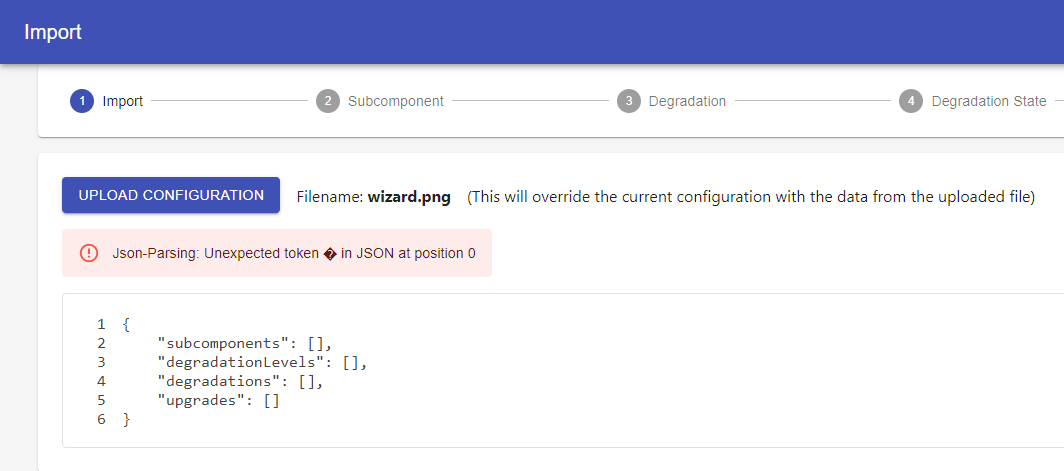
\includegraphics[width=\textwidth]{img/import_invalid_file.png}
    \caption{Import invalid file}
    \label{fig:import_invalid_file}
\end{figure}

\noindent The second part of the validation is the validation of the JSON data itself. The JSON data requires several properties to be a valid configuration. Details on this part of the validation can be found in section \ref{sec:validation}.
The found problems of the second part of the validation will also be displayed. An example can be seen in figure \ref{fig:import_invalid_json} where there are several problems with the imported object. If a problem occurs for an element of an array, for example in the subcomponents, the index of the element will also be added to the error message. This will help a user to identify the problem and update it accordingly.

\begin{figure}[ht]
    \centering
    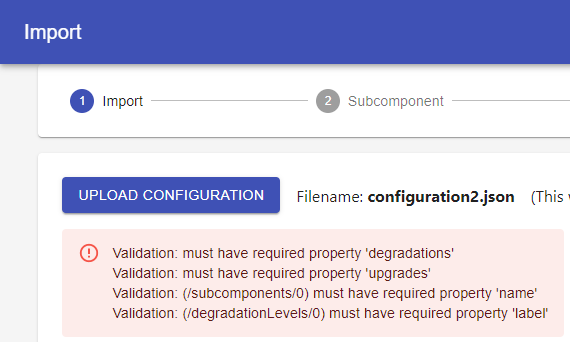
\includegraphics[width=0.8\textwidth]{img/import_invalid_json.png}
    \caption{Import invalid JSON}
    \label{fig:import_invalid_json}
\end{figure}

\section{Validation}
\label{sec:validation}

The validation of the configuration at the import is a central part of the application, because it enforces a valid configuration. A validation at another point in the configuration is not necessary because all current wizard steps leave the global configuration in a valid state.

For the validation the \textit{ajv JSON schema validator}\footnote{\url{https://github.com/ajv-validator/ajv}} was used, because it has several advantages over a custom implementation. A custom implementation requires not only to write the complete parsing logic, but also has to be adapted if changes to the configuration schema are required in the future. The configuration schema is a description of all the properties a JSON object has to have to be a valid configuration.

There are two popular schema languages that allow the definition of JSON data. On the one hand there is the \textit{JSON schema}\footnote{\url{https://json-schema.org/}} and on the other hand there is the \textit{JSON Type Definition}\footnote{\url{https://datatracker.ietf.org/doc/html/rfc8927}}. Both schema description languages are supported by ajv, but the decision was made in favor of the JSON schema. Although there is an RFC for the JSON Type definition and only a draft for JSON Schema, the JSON Schema is better supported in the industry \cite{ajv_comparison}. Since both are supported by ajv, the decision was made to use JSON Schema because of the better support, but this can easily be changed in the future to the JSON Type Definition.

The change from the JSON Schema to the JSON Type Definition is for this application quiet simple, because you just have to replace the schema file and adapt the configuration of ajv, which can be found in src\textbackslash util\textbackslash

\subsection{JSON schema}
This section provides a short overview of the configuration schema, the complete definition can be found in the provided source code. For a better understanding of the JSON configuration schema a mapping to an er-diagram with highlighted parts is shown in figure \ref{fig:configuration_diagram}.

\begin{figure}[ht]
    \centering
    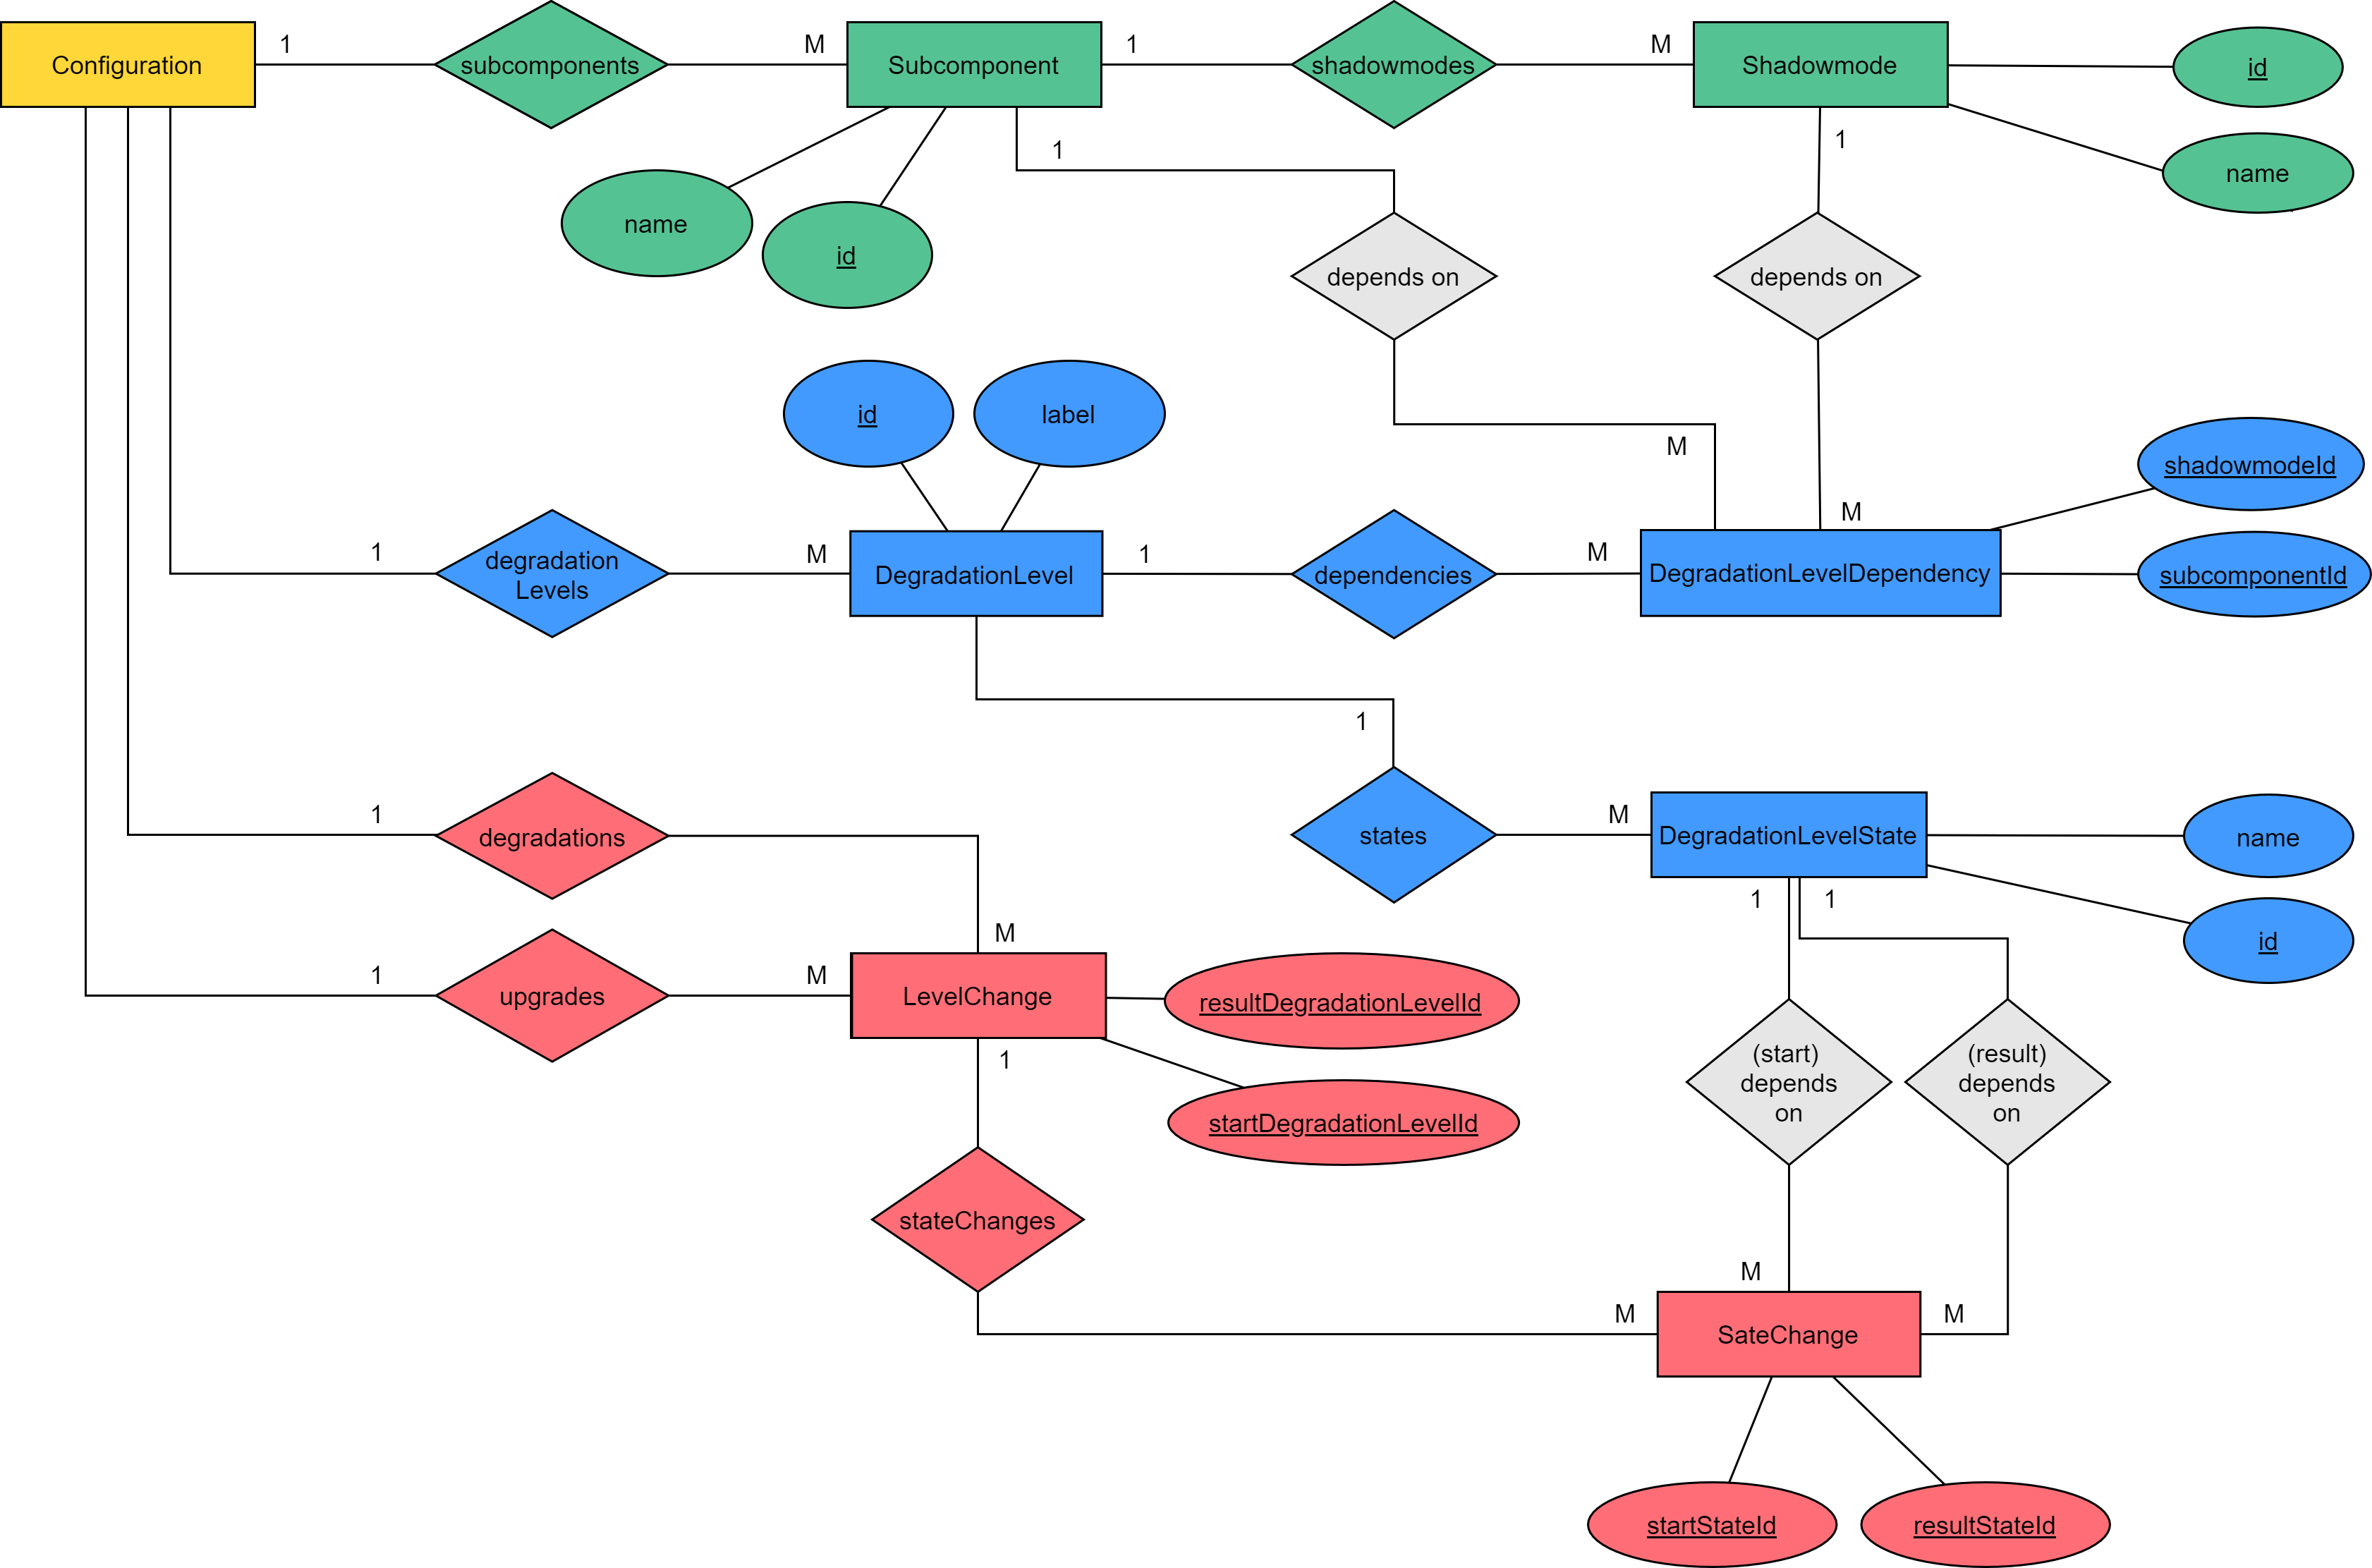
\includegraphics[width=\textwidth]{img/configuration_diagramm.png}
    \caption{JSON configuration schema mapped on an er-diagram}
    \label{fig:configuration_diagram}
\end{figure}

\noindent The first important part of a configuration are the subcomponents. A system consists of several subcomponents that are relevant for the degradation/upgrade. The subcomponents are stored in an array in the configuration and highlighted in green in figure \ref{fig:configuration_diagram}. Each subcomponent has a set of shadowmodes that are all the operational states a subcomponent can have. For example the typical states are an \textit{On}-state or an \textit{Off}-state.

The next part of the configuration are the degradation levels which represent the levels in which the system can be. In figure \ref{fig:configuration_diagram} all relevant parts that are related to the degradation levels are highlighted with blue. A degradation level is active when one of the attached sets of dependencies is true. A dependency set is true when all the relevant subcomponents are in the specified shadowmodes or in other words when the subcomponents run in a defined state that matches the dependencies of the degradation level. For example a degradation level can depend on a crucial part of the system and that this part is in the On-state. If it is not in the On-state a degradation into another level has to be done. In order to be able to not only define a single set of dependencies, it is possible to add several sets of dependencies. Each set represents a state of the system, or more precise the state of some subcomponents, in which they have to be in. If one of the sets of a degradation level fits the current system state, this degradation level is the active degradation level. Only the subcomponents and the states that are relevant for a degradation level are stored in the dependency array of a set. The \textit{don't care}(DC) cases will be ignored to save storage space. The degradation level states are the internal states of each degradation level. They describe the states the state machine of each degradation level can be in.

The final and central part of the configuration is the upgrade and degradation specification of the system, in figure \ref{fig:configuration_diagram} highlighted in red. Both the upgrade and the downgrade from on degradation level to another degradation level can be represented as level change. A level change object consists of the degradation level where the change starts and where it results in. A simple example could be a system that starts at the Off-state and after an upgrade results in the On-state (on system level, not on subcomponent level). In addition to the level change, it is also required to define in what internal state the start and the result degradation level has to be. In order to map the states each level change contains a set of mapping of the states of the start and result degradation level.

The grey highlighted parts in figure \ref{fig:configuration_diagram} represent relations between the different aspects of the configuration. They are implemented using the ids of the relevant objects and therefore create internal dependencies. This is an important for the application, because due to these dependencies, it is required to update the global configuration when a related object is updated or deleted. For example if you delete a subcomponent or change it's id, the changes have to be propagated and for example the dependencies in the degradation levels updated or deleted.

\section{Subcomponent configuration}

The subcomponent configuration is the first step when a user starts the wizard without importing an existing configuration. Otherwise it is the second step that allows the adjustment of the imported subcomponents.
This component offers a table that displays all defined subcomponents and allows to sort and navigate through them. In addition, this component allows the creation, update or deletion of them. In figure \ref{fig:subcomponent_view} an example is shown with several defined subcomponents.

\begin{figure}[ht]
    \centering
    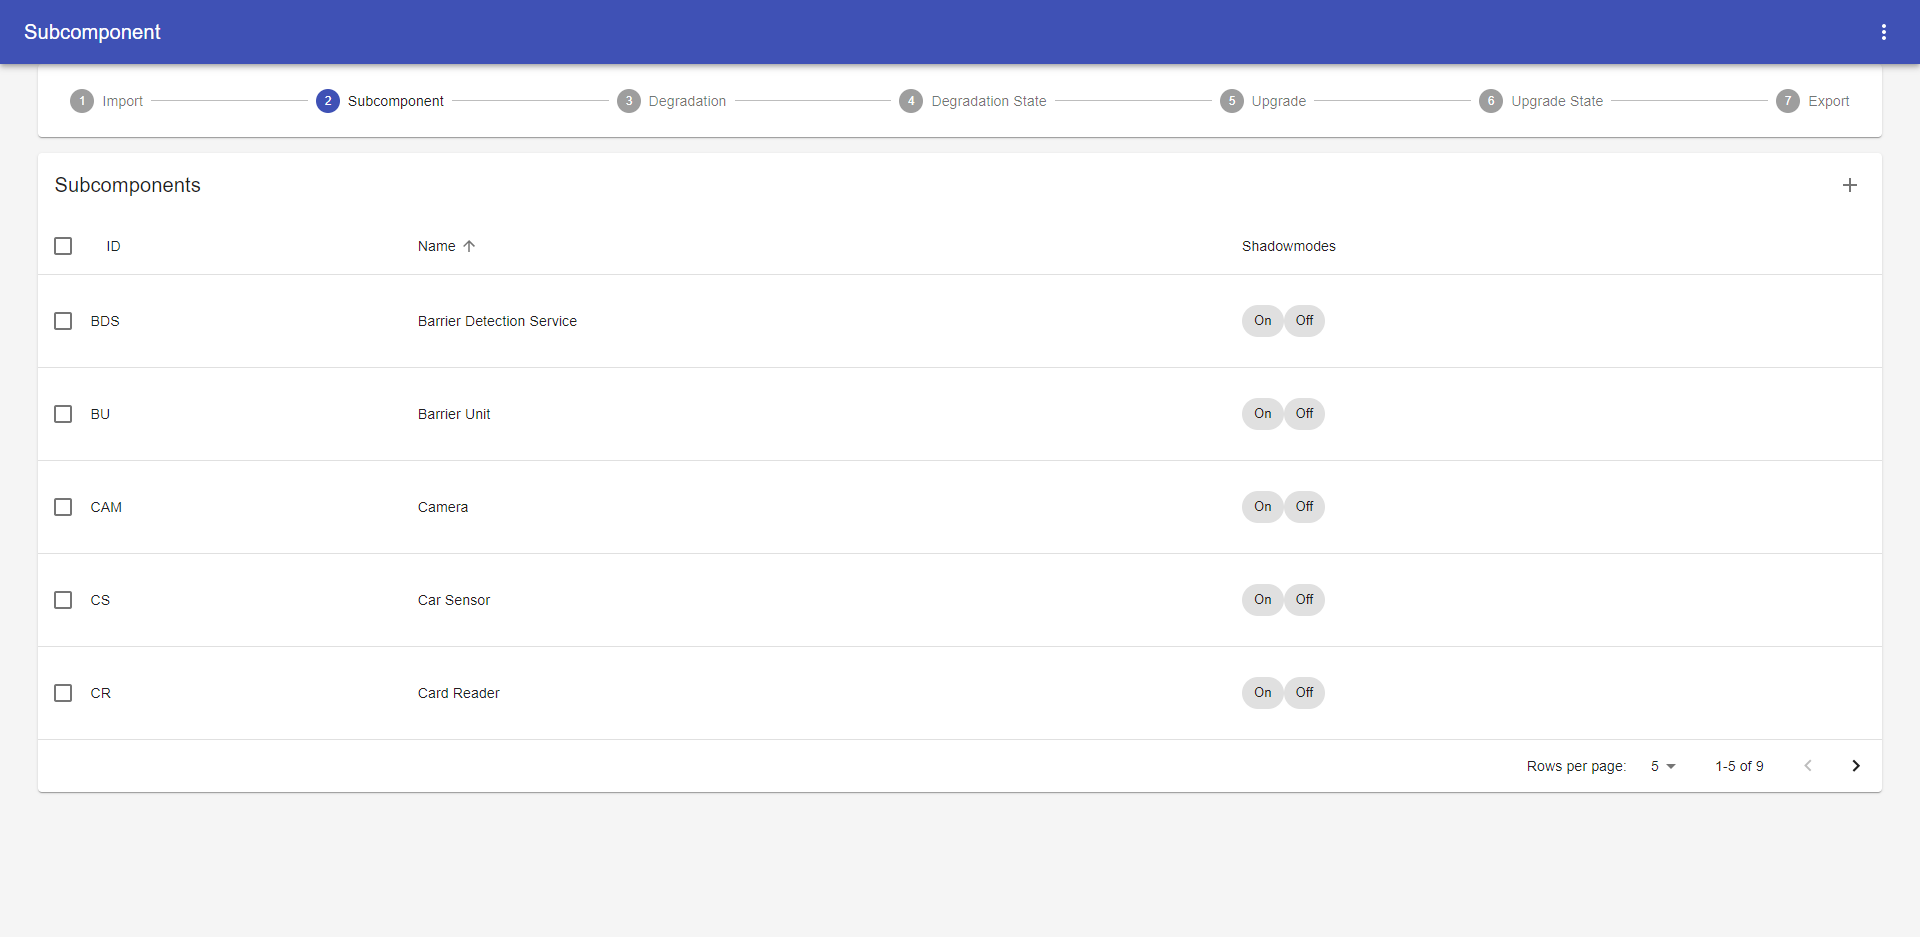
\includegraphics[width=\textwidth]{img/subcomponents_overview.png}
    \caption{Subcomponent view}
    \label{fig:subcomponent_view}
\end{figure}

The table allows to select subcomponents and depending on the amount of selected subcomponents different actions are possible. If only one subcomponent is selected it is possible to delete or edit the selected one or to create a new subcomponent (compare figure \ref{fig:subcomponent_view_single} on the top right corner of the table).

\begin{figure}[ht]
    \centering
    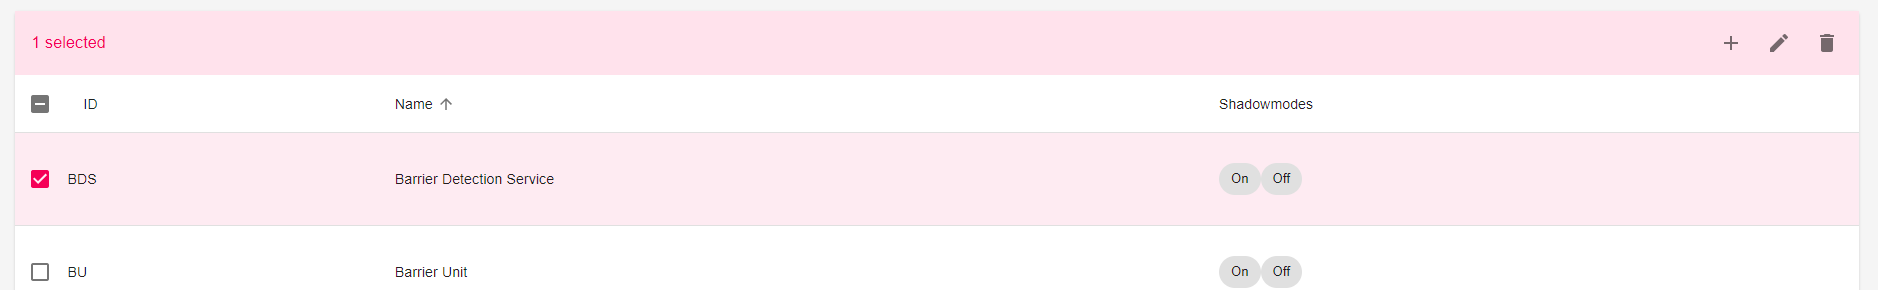
\includegraphics[width=\textwidth]{img/subcomponents_single_select.png}
    \caption{Subcomponent single selection}
    \label{fig:subcomponent_view_single}
\end{figure}

If a user selects multiple subcomponents it is only possible to delete all of them or to create a new one. (compare figure \ref{fig:subcomponent_view_multi}).

\begin{figure}[ht]
    \centering
    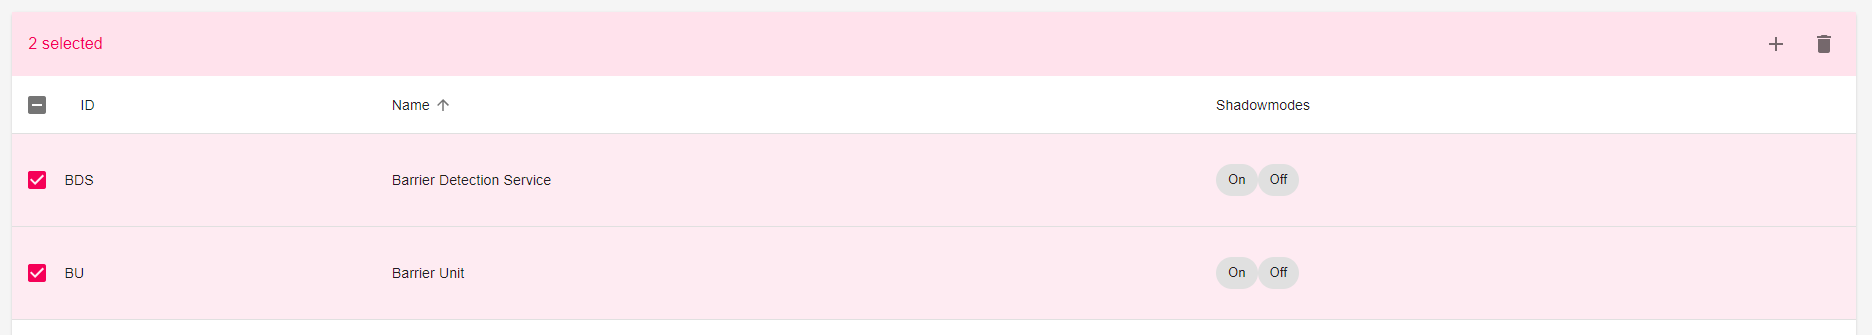
\includegraphics[width=\textwidth]{img/subcomponents_multi_select.png}
    \caption{Subcomponent multi selection}
    \label{fig:subcomponent_view_multi}
\end{figure}

For the deletion, the creation and the update of a subcomponent different dialogs are displayed.
The deletion dialog is shown in figure \ref{fig:subcomponent_delete_dialog} and shows the amount of subcomponents that will be deleted. The deletion of one or more subcomponent will also delete the references that exist in other components. For example a degradation level depends on a subcomponent and therefore has a degradation level dependency object that will be deleted too.

\begin{figure}[ht]
    \centering
    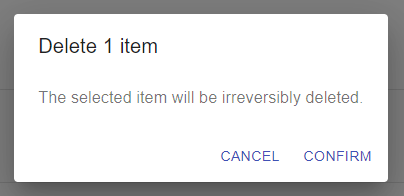
\includegraphics[width=0.7\textwidth]{img/subcomponents_delete.png}
    \caption{Subcomponent delete dialog}
    \label{fig:subcomponent_delete_dialog}
\end{figure}

The create and edit dialog will allow to create or edit a subcomponent. If no name is set for a subcomponent the dialog will autofill the id with the value of the name. In addition to this the dialog will validate if there are empty fields and if another subcomponent already exists with the id set in the dialog. This can be the case when either a new component is created with an existing id or the id of an existing one is changed. Changing the id of an existing subcomponent will also update the dependencies of the degradation levels that depend on this subcomponent. An example of the create dialog is shown in figure \ref{fig:subcomponent_create_dialog}. For each subcomponent it is required to define one or more shadowmode and therefore a custom input was designed. This input allows to enter a value in the text field and after the "enter" button is pressed the value will be added as chip on the right side. For example the \textit{On} or \textit{Off} shadowmodes in figure \ref{fig:subcomponent_create_dialog}. For the creation of a new subcomponent a default shadwomode \textit{Off} is set. Deleting a shadowmode will also update the degradation level dependencies that rely on this shadowmode.

\begin{figure}[ht]
    \centering
    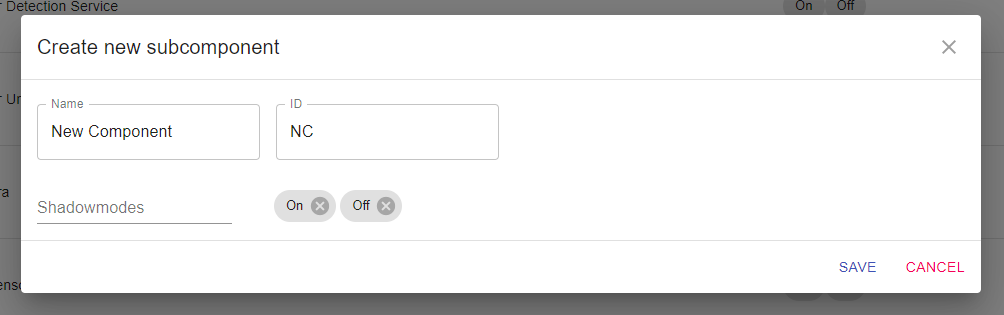
\includegraphics[width=\textwidth]{img/subcomponents_create.png}
    \caption{Subcomponent create dialog}
    \label{fig:subcomponent_create_dialog}
\end{figure}

\section{Degradation Level Management}
The creation, update and deletion of degradation levels is combined with the functionality to define upgrades and degradations, as described in section \ref{sec:deg_and_upg}. The degradtion level tree allows to select single and multiple degradation levels and depending on that there are different actions possible. If only one is selected there are three possible actions: creating a new degradation level, edit the selected one or delete the selected one (compare figure \ref{fig:degradation_crud_level_single}). The selection of multiple degradation levels (compare figure \ref{fig:degradation_crud_level_multi}) allows only the deletion of the selected levels or the creation of a new level. The deletion for both cases will display a dialog similar to the one shown in figure \ref{fig:subcomponent_delete_dialog}.

\begin{figure}[ht]
    \centering
    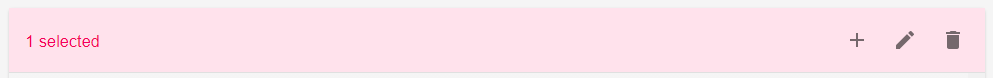
\includegraphics[width=\textwidth]{img/degradation_level_crud_single.PNG}
    \caption{Degradation level single selection}
    \label{fig:degradation_crud_level_single}
\end{figure}

\begin{figure}[ht]
    \centering
    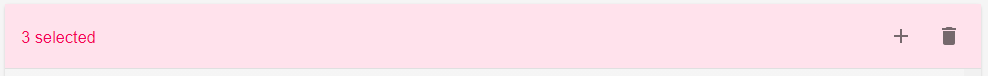
\includegraphics[width=\textwidth]{img/degradation_level_crud_multi.PNG}
    \caption{Degradation level multi selection}
    \label{fig:degradation_crud_level_multi}
\end{figure}

The creation and edit dialog (shown in figure \ref{fig:degradation_level_dialog}) allows to either create or edit a degradation level. The dialog will validate the id to enforce unique ids for each degradation level in the configuration. Depending on the subcomponents that are already defined, the dropdown selection inputs will be generated dynamically. These dropdown selection inputs allow to define the dependencies of the degradation level by selecting a shadowmode for each subcomponent. If the shadowmode is set to \textit{DC} (don't care) then no value will be created in the configuration (or an existing value will be deleted in the edit case). The internal states are a custom input that allows again to add a state for degradation level by entering a string and pressing enter. After the enter button was pressed the state will be added as chip on the right and can be deleted with the X-button. 
The deletion of the states of a degradation level will also trigger an update of the configuration and will remove all references that require the state (the state changes).

\begin{figure}[ht]
    \centering
    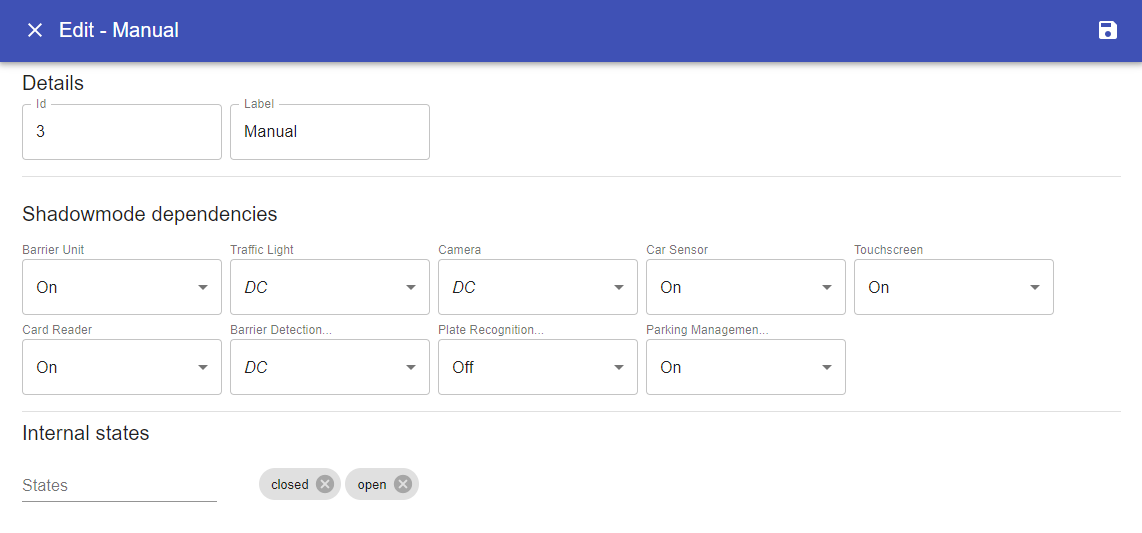
\includegraphics[width=\textwidth]{img/degradation_level_dialog.png}
    \caption{Degradation level dialog}
    \label{fig:degradation_level_dialog}
\end{figure}

\section{Degradation and Upgrade configuration}
\label{sec:deg_and_upg}

The second part of the degradation level configuration is the specification of the degradations and upgrades. In order to be able to specify the hierarchy of the degradation levels a custom component was created that allowed to drag and drop the degradation levels into a tree structure.

An example for a possible degradation is shown in figure \ref{fig:degradation_level_tree} that also shows several features. All unsorted degradation levels will be displayed in a sidebar and can be tracked to any position in the tree. If there is no unsorted degradation level left, the sidebar will not be displayed. The selection can vary from one to many selected degradation levels whereby the degradation levels can be in the tree and the sidebar at the same time. An example for the selection is also shown in figure \ref{fig:degradation_level_tree} where the selection is highlighted in red. In order to remove a degradation level from the tree it is possible to drag the node onto the delete zone at the top. This will remove the degradation or upgrade from the configuration. The degradation level will be added as unsorted degradation level again. The OFF degradation level will always be the top node in the tree and can't be removed or changed. It will have as id '0' and won't explicitly be saved in the configuration.

\begin{figure}[ht]
    \centering
    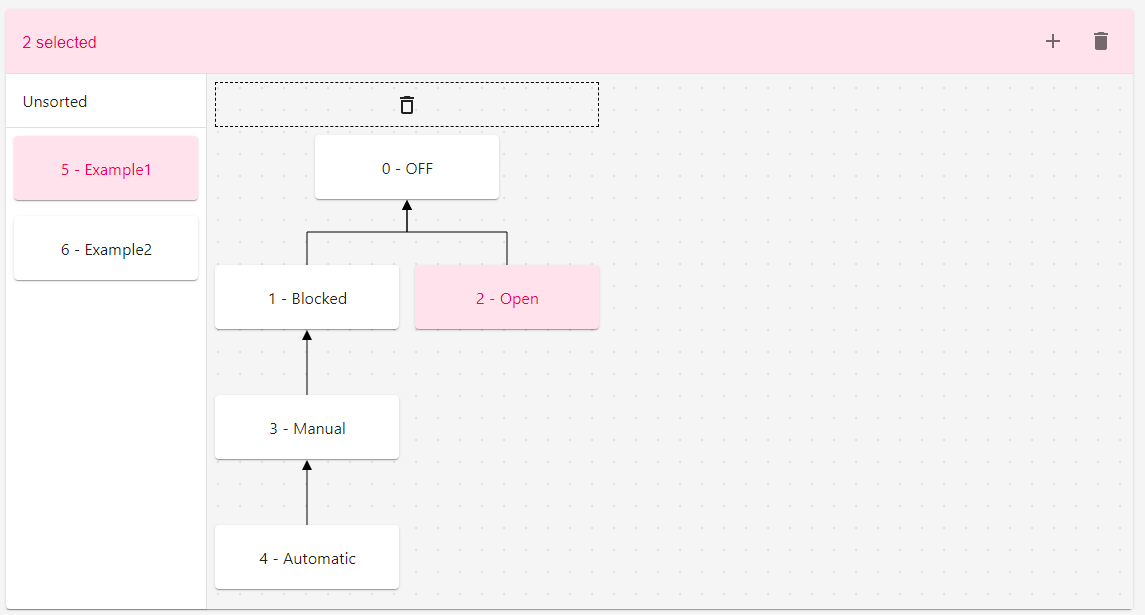
\includegraphics[width=\textwidth]{img/degradation_tree.png}
    \caption{Degradation level tree}
    \label{fig:degradation_level_tree}
\end{figure}

The tree allows to insert (drag and drop) degradation levels above or below a sorted level. In figure \ref{fig:degradation_level_tree_drop} an example for the drop above and below a degradation level in the tree is shown. Hovering over the drop zone (above or below of a node in the tree) will highlight the zone in blue and allows to add the dragged degradation level at this position. 

\begin{figure}[ht]
    \centering
    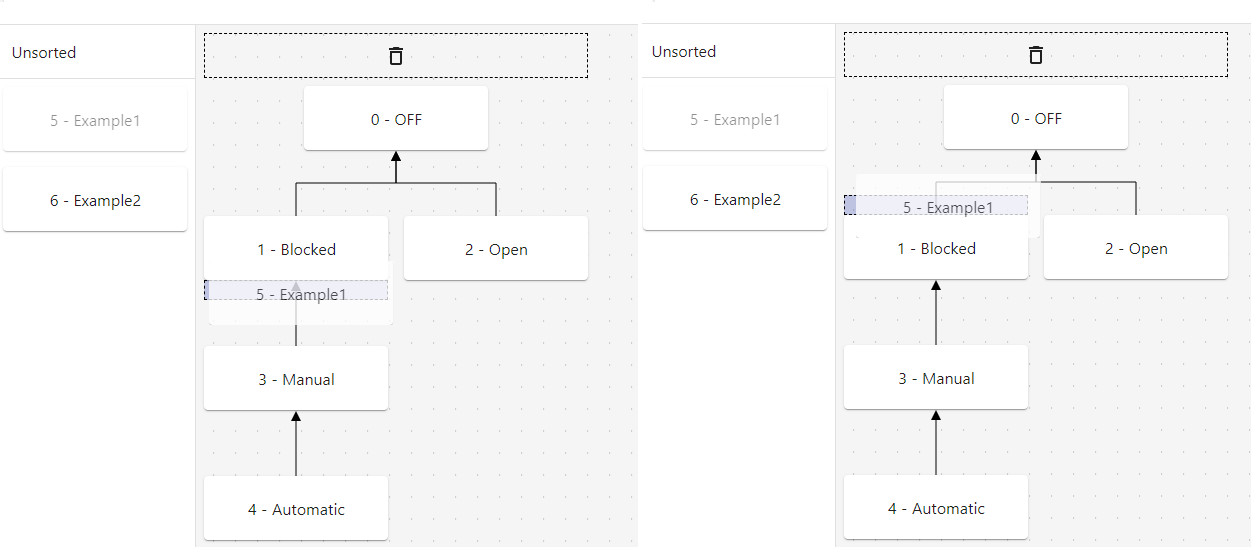
\includegraphics[width=\textwidth]{img/degradation_tree_drop.png}
    \caption{Degradation level tree drop behavior (left: below, right: above)}
    \label{fig:degradation_level_tree_drop}
\end{figure}

Changing the position of a degradation level will reset the configuration or more precise the level change itself. The level changes stores the start and result state of the degradation levels that have to be configured again in the next view. Inserting the node above another one will therefore update the level changes (degradation or upgrade) for the already connected degradation levels, but reset the state changes.

The tree show up to this point is used to define the degradations, but allows not to specify the upgrades. For the upgrades the tree will show an inverse version, which means that the arrows will not start from a degradation level and point in the direction of the OFF degradation level. Instead the arrows will point starting from the OFF degradation level to the child nodes.
The specification of the upgrades will be therefore done in a separate step in the wizard that allows a completely independent configuration from the degradations. In order to simplify the process, there is an additional button that allows the automatic creation of the upgrade tree based on the already specified degradations tree. The button, in figure \ref{fig:upgrade_level_tree_drop} in the sidebar on the top right, will open a confirmation dialog that will ask a user to confirm the changes. After the confirmation the previous upgrade tree will be deleted and the inverse of the degradation tree will be calculated and saved in the configuration as new upgrade tree. An important note is here, that both of the trees can be changed independently (before and afterwards the auto creation) and it is therefore possible to create two completely different trees. This explains also why the configuration contains two separate arrays for the tree configuration: one for the upgrades and one for the degradations. In contrast to this, the deletion/update or creation of a degradation level will influence both trees. For example the change of the id of a degradation level will update the id in both the upgrade and the degradation tree.

\begin{figure}[ht]
    \centering
    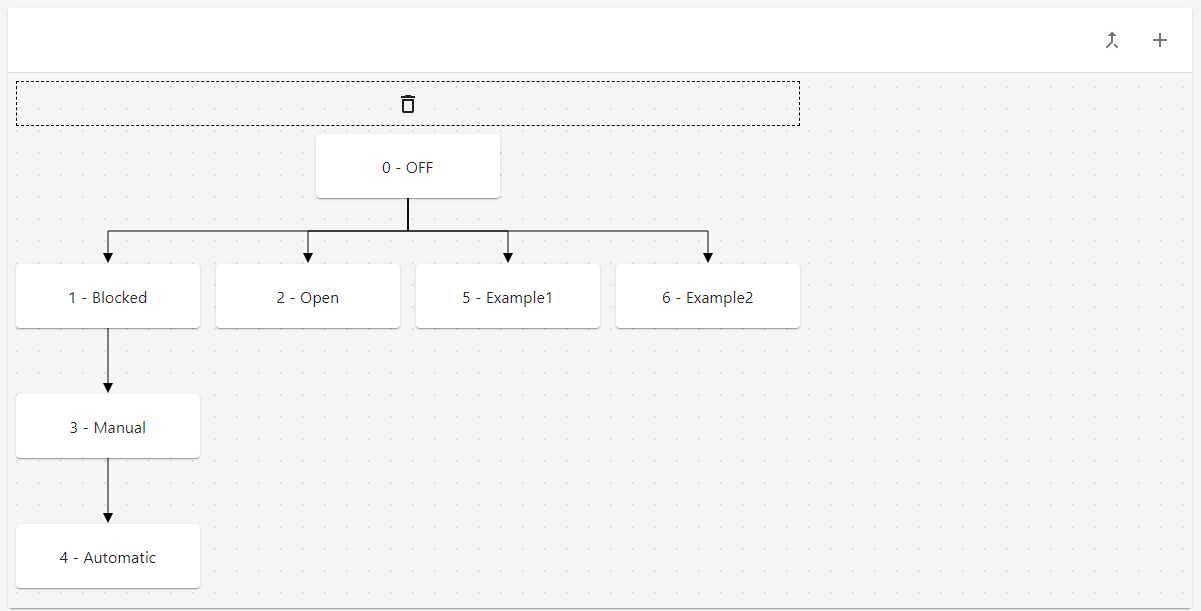
\includegraphics[width=\textwidth]{img/upgrade_tree.png}
    \caption{Upgrade degradation level tree}
    \label{fig:upgrade_level_tree_drop}
\end{figure}

\section{LevelChange configuration}
Another important part for the configuration is the specification of the states the level changes start and result in. To realize this, every level change contains a set of state changes which will contain the start and result state of the involved degradation levels. In order to configure these states another component was implemented that allows to define the result state for each start state of a level change. Since there are level changes for the upgrades and the downgrade, the configuration for these states have to be done for both cases and therefore these are two independent steps in the wizard. Example for the degradation state changes can be found in figure \ref{fig:deg_state_change} and examples for the upgrade state changes in figure \ref{fig:upg:state_change}. 

\begin{figure}[ht]
    \centering
    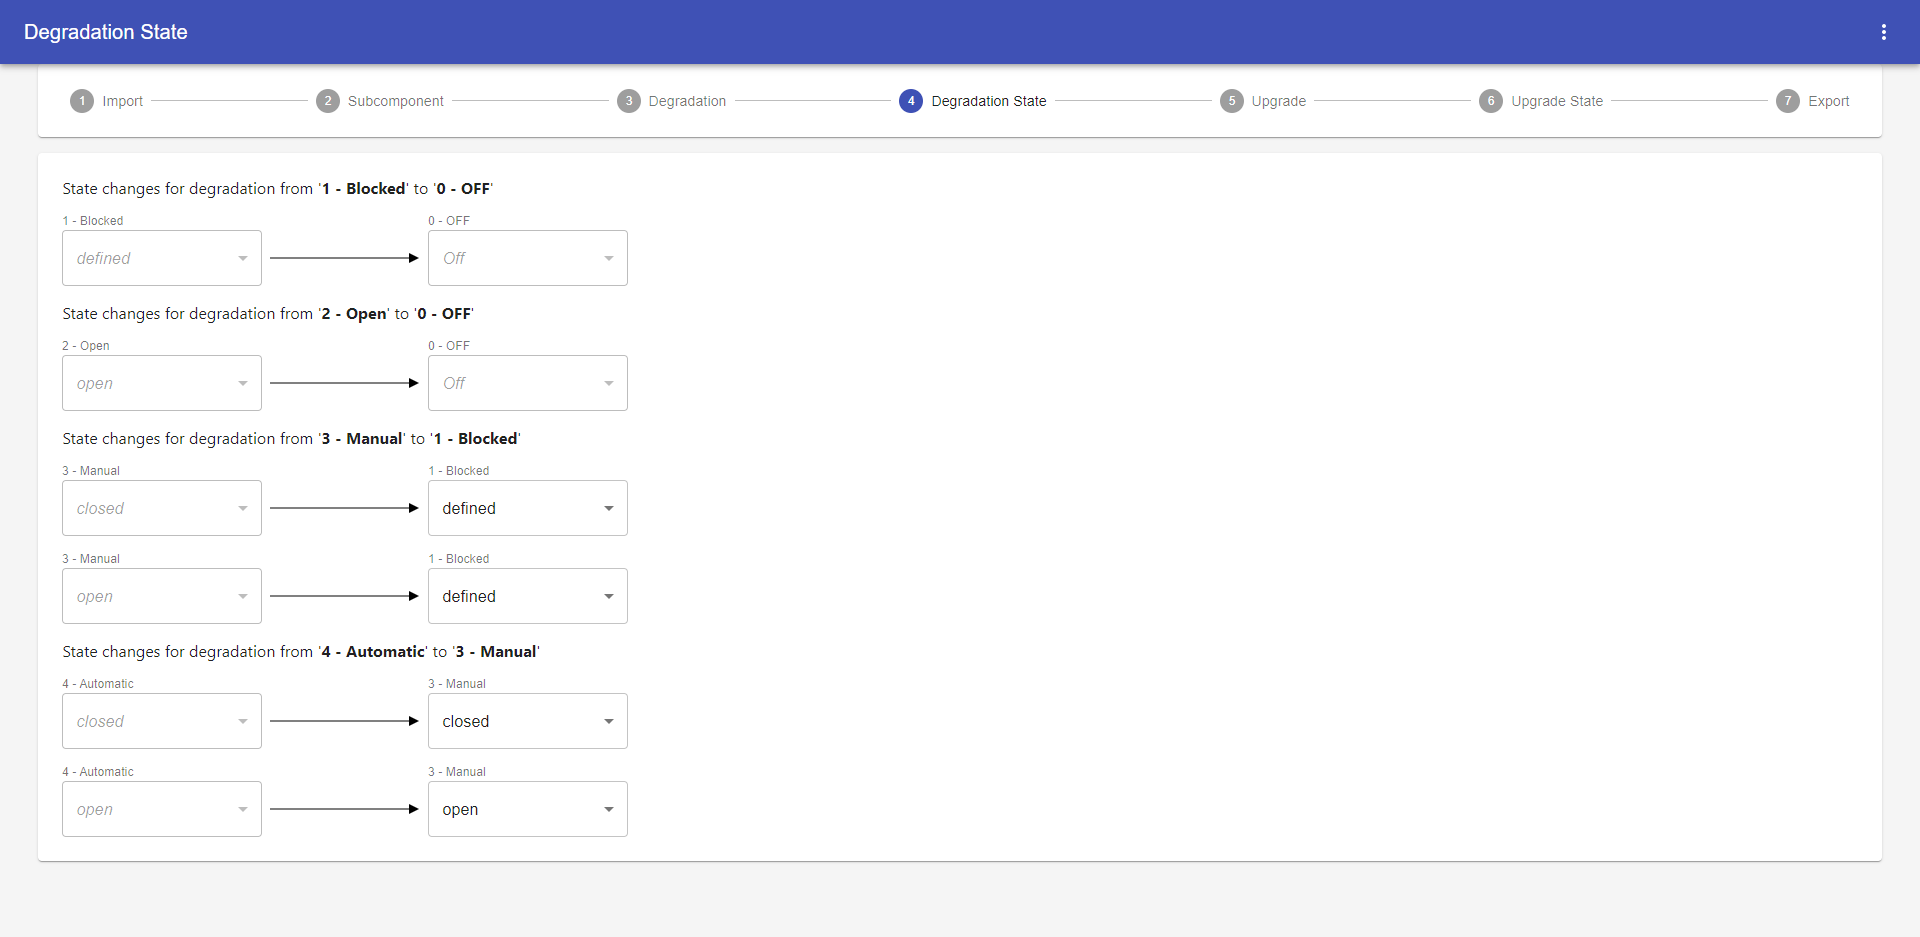
\includegraphics[width=\textwidth]{img/degradation_level_change_states.png}
    \caption{Degradation state change configuration}
    \label{fig:deg_state_change}
\end{figure}

\begin{figure}[ht]
    \centering
    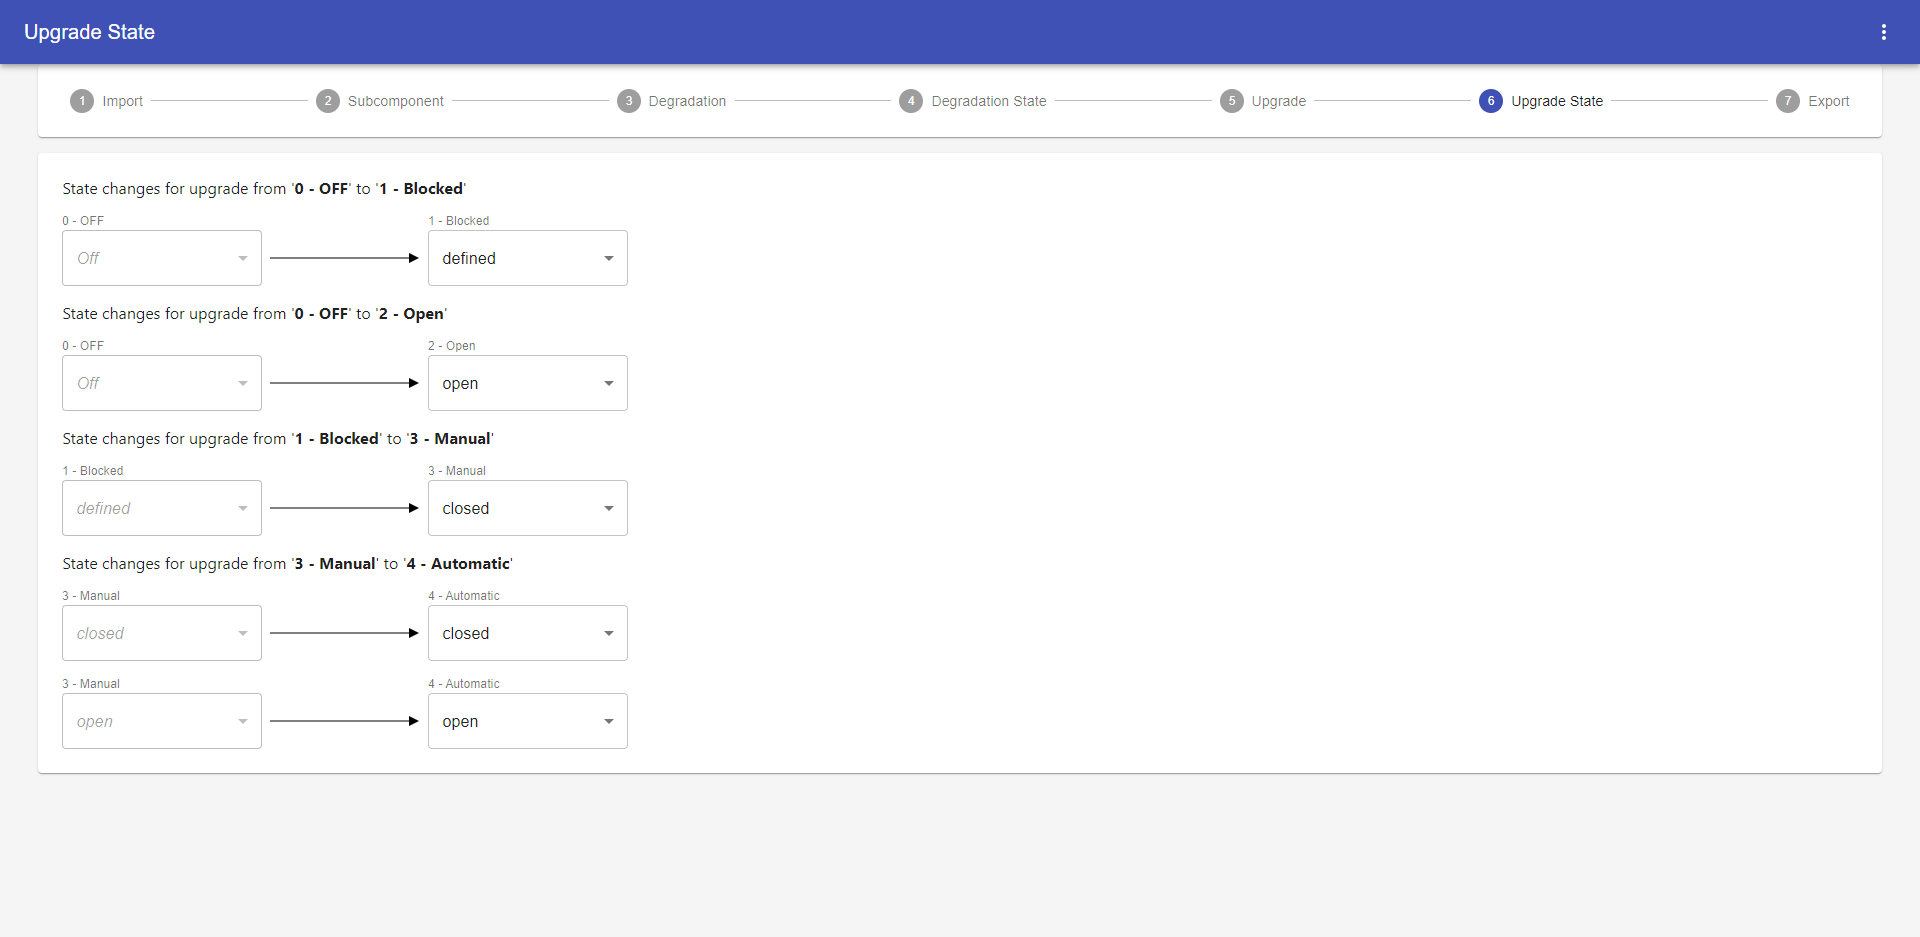
\includegraphics[width=\textwidth]{img/upgrade_level_change_states.png}
    \caption{Upgrade state change configuration}
    \label{fig:upg:state_change}
\end{figure}

\newpage

\section{File structure}
This section will give a short overview of the file structure of the project to facilitate further enhancements:

\dirtree{%
.1 root.
.2 docs.
.2 examples.
.2 public.
.2 src.
.3 components.
.3 context.
.3 models.
.3 util.
}\hfill

The docs directory contains the documentation for this project, like this report. The examples folder contains example files for the configuration. In the public folder the public resources for the web application are stored. For example the favicon or the index.html.

The src folder contains the application that consists of different parts. In components folder are all components of the application which means their typescript files as well as their css files. Each component has its own folder that contains these files as well as other sub components. For example the importView contains a component for the file import. The context folder contains the definition of the configuration context that is used to store the current configuration on application level. The models folder contains a set of interfaces that describe the configuration and its components to allow validating the typescript code. There is a set of different functionalities in the util folder that help to solve some general problems, for example the validator for the schema with the corresponding schema description file.

\clearpage